\documentclass[11pt]{article}

\usepackage[a4paper,margin=1in]{geometry}
\usepackage[T1]{fontenc}
\usepackage{newtxtext,newtxmath}
\usepackage{graphicx}
\usepackage{booktabs}
\usepackage{amsmath}
\usepackage{float}
\usepackage[colorlinks=true,linkcolor=black,citecolor=black,urlcolor=blue!50!black]{hyperref}
\usepackage[font=small,labelfont=bf]{caption}
\usepackage{titlesec}
\usepackage{abstract}
\usepackage{authblk}

\titleformat{\section}{\normalfont\large\bfseries}{\thesection}{0.7em}{}
\titleformat{\subsection}{\normalfont\bfseries}{\thesubsection}{0.7em}{}
\titlespacing*{\section}{0pt}{1.6em}{0.7em}
\titlespacing*{\subsection}{0pt}{1.2em}{0.5em}

\renewcommand{\abstractnamefont}{\normalfont\bfseries}
\renewcommand{\abstracttextfont}{\normalfont\itshape}

\title{\vspace{-1em}Exact Symplectic Reduction for Quantum Circuits:\\
A Cost-Aware Engine and a Diagnostic Study of\\
Database Coverage Limits}
\author[1]{Arnav Kapoor}
\affil[1]{Indian Institute of Science Education and Research Bhopal}
\date{}

\begin{document}
\maketitle
\vspace{-2.5em}

\begin{abstract}
\noindent
We present an exact, tolerance-free engine for local term-replacement
circuit reduction on Clifford gate sets, together with a two-qubit-aware
search objective and a deterministic block-reordering pass that
diversifies local search without displacing its stochastic component. The
engine keys a compute graph of reachable unitaries by a bit-exact signed
symplectic tableau rather than by a numerical tolerance, so every
replacement it finds is correct by construction. On a four-qubit,
length-300 ion-trap benchmark protocol, this reduces circuits to a mean of
$66.7\pm12.9$ gates and $25.9$ two-qubit gates, improving on the strongest
previously published result for the same protocol by 40\% and 40\%
respectively ($p<10^{-45}$, one-sample $t$-test, $n=100$). On a NISQ gate
set outside the reach of the exact engine, a numerical-tolerance variant of
the same search infrastructure trails that published result, and we treat
the shortfall as the central object of study rather than an incidental
weak point. Six candidate explanations, including compute-graph depth
tested independently on both the three-wire and four-wire graph, are each
tested by direct experiment and ruled out in turn, localizing the gap to
a database factorization limit that is not resolved by depth along either
axis. Two further candidates fare no better: a node-keying fragility that
under-merges 21--32\% of compute-graph nodes is real and fixed but changes
the NISQ result by nothing, and a bidirectional reach-extension technique
finds genuine additional matches but costs more search time than it saves.
A ninth attempt breaks the pattern: porting the original MATLAB reference
implementation's own reduction loop verbatim -- rejection-sampled,
narrow-wire random windows tried at far higher raw throughput than an
exhaustive sweep, in exchange for much weaker per-attempt mechanics --
improves the NISQ mean by $3.4\%$ ($p<10^{-23}$, paired $t$-test, $n=100$)
over the exhaustive sweep it replaces, and is adopted as the new default;
it narrows the published gap slightly without closing it, and is reported
as a real, modest, load-bearing finding rather than a resolution.
Benchmarking the deeper four-wire graph exposed an engineering
defect general enough to be worth reporting on its own: caching a
disk-backed compute graph per worker process rather than per task, under
process-parallel search, changes measured search cost by two orders of
magnitude and can invert a benchmark's conclusion. A third, richer
ion-trap pool mixing Clifford and non-Clifford rotations ($\pm\pi/2$,
$\pm\pi/4$, $\pm\pi/8$) exposes a boundary condition neither protocol
reveals alone: its branching factor forces much shallower compute graphs
under the same build budget, and at that depth the method loses even to a
generic transpiler, directly demonstrating that the approach's edge is
a direct trade against pool size, not a free property of the technique.
\end{abstract}

\noindent\textbf{Keywords:} quantum circuit optimization, transpilation,
Clifford group, compute graphs, local search, benchmarking

\section{Introduction}
\label{sec:intro}

Every quantum circuit eventually has to run on hardware that supports a
small, fixed set of native gates, and the translation from an algorithm's
natural gate set to that native set, decomposition followed by mapping
followed by scheduling, routinely leaves behind redundancy that a human
reading the resulting sequence would remove on sight: a rotation
immediately undone by its inverse, two rotations about the same axis that
should have been one, a two-qubit gate sandwiched between single-qubit
gates that commute straight through it. On present-day noisy
intermediate-scale quantum (NISQ) hardware, where every additional gate is
additional exposure to decoherence and two-qubit gates dominate both error
rate and duration \cite{Preskill2018NISQ,Arute2019Supremacy,Cross2019QuantumVolume},
closing this gap between what a circuit does and how many gates it takes to
do it is not an optimization but a precondition for getting a usable result
at all.

Circuit optimization has accordingly been attacked from several directions:
peephole and template-matching rewriting over fixed gate identities
\cite{Nam2018Automated,Amy2014TDepth,ZulehnerPalerWille2018}, structural
compilation pipelines tuned to a specific device topology
\cite{Maslov2017IonTrap,Murali2020TrappedIon,BlumRoli2003Metaheuristics},
production transpilers that combine many such passes behind a single
interface \cite{JavadiAbhari2024Qiskit,Sivarajah2020Tket,Younis2021BQSKit},
and, more recently, architecture-search methods that treat the mapping or
the circuit itself as an object to be searched over with learned or
evolutionary methods
\cite{Martyniuk2024QASSurvey,Zhu2023QASSurvey,Zhang2021NeuralPredictorQAS,Zhang2022DifferentiableQAS,He2024TrainingFreeQAS,Brandhofer2021Rydberg,Datta2022_2DMapping,Datta2022_HexMapping}.
Rosenhahn, Osborne and Hirche's local term-replacement scheme sits closer
to the first category, but with a distinctive mechanism: rather than
matching a fixed library of hand-derived identities, it precomputes, for a
given gate pool and search depth, a compute graph of every unitary reachable
from the identity together with the shortest token chain that realizes it,
then repeatedly samples circuit blocks and substitutes the graph's stored
chain whenever it is shorter than the block itself
\cite{Rosenhahn2025Optimization}, building on the same group's earlier
Monte Carlo graph search work \cite{RosenhahnTobias2023MCGS}. Matched
against a $10^{-5}$ numerical tolerance, this reaches substantial
reductions on an ion-trap gate set (RX, RY, RZ, RXX) and a NISQ gate set
(RX, RZ, CZ), and the paper shows the effect measurably on real IBM
hardware.

\section{Related work}
\label{sec:related}

\paragraph{Structural and template-based rewriting.} Classical logic
minimization has a long history of local rewrite rules, and quantum
circuit optimization inherited the idea directly: T-depth and T-count
reduction via matroid partitioning over Clifford+T circuits
\cite{Amy2014TDepth}, automated peephole optimization of large
parametrized circuits by commutation and gate fusion
\cite{Nam2018Automated}, and device-specific compilation pipelines for
trapped-ion \cite{Maslov2017IonTrap} and superconducting
\cite{ZulehnerPalerWille2018} hardware all locally rewrite a circuit
against a fixed or semi-fixed rule set. The compute-graph approach we
build on generalizes this by deriving its rewrite rules from an exhaustive
search over a gate pool rather than from hand-picked identities, at the
cost of the search itself being the bottleneck; general treatments of
local and metaheuristic search over combinatorial structures
\cite{BlumRoli2003Metaheuristics} apply directly to characterizing that
cost.

\paragraph{Transpilers and toolkits.} Qiskit \cite{JavadiAbhari2024Qiskit},
t$|$ket$\rangle$ \cite{Sivarajah2020Tket}, and the Berkeley Quantum
Synthesis Toolkit \cite{Younis2021BQSKit} are the three baseline compilers
against which the paper we build on, and consequently this paper, are
evaluated. All three combine many optimization passes, commutation-based
gate cancellation, template matching, numerical resynthesis of small
blocks, behind a single interface, and BQSKit in particular treats
resynthesis as a numerical optimization problem over a topology-aware
search \cite{Davis2020TopologyAware} that is later reorganized
hierarchically \cite{Wu2021HierarchicalSynthesis}. None of the three build
an explicit compute graph keyed for exact reuse across circuits the way
the method here does; the tradeoff is a slower, offline-amortized search
against a faster, per-circuit one.

\paragraph{Quantum architecture search.} A parallel literature treats the
choice of circuit, or the choice of hardware mapping for a fixed circuit,
as a search or learning problem: neural-predictor-guided search
\cite{Zhang2021NeuralPredictorQAS}, differentiable relaxations
\cite{Zhang2022DifferentiableQAS}, training-free proxies
\cite{He2024TrainingFreeQAS}, and genetic and random-search variants
\cite{Rasconi2019GeneticCompilation,Ashhab2024RandomSearch}, surveyed
broadly in \cite{Martyniuk2024QASSurvey,Zhu2023QASSurvey}. Mapping-specific
work targets particular topologies: Rydberg-atom arrays
\cite{Brandhofer2021Rydberg}, two-dimensional and hexagonal nearest-neighbor
grids \cite{Datta2022_2DMapping,Datta2022_HexMapping}, and multi-qubit
trapped-ion architectures with shuttling \cite{Murali2020TrappedIon}. The
present work sits at the circuit-rewriting end of this spectrum rather
than the mapping end, but shares its reliance on random-forest classifiers
\cite{Breiman2001RandomForests} and reinforcement learning
\cite{Wauters2020RLOptimization} as cheap proxies that gate an expensive
exact evaluation, the role a random-forest classifier plays in the V3
variant of the method we benchmark against and in our own reimplementation
of it (Section~\ref{sec:sampling}).

\paragraph{Exact simulation and the Clifford group.} The exact engine in
Section~\ref{sec:exact} rests on the stabilizer formalism: the observation
that Clifford circuits are efficiently classically simulable by tracking
the evolution of Pauli operators rather than state vectors
\cite{Gottesman1998Heisenberg}, made practical at scale by the
tableau-based simulation algorithm of Aaronson and Gottesman
\cite{AaronsonGottesman2004}, and given a canonical decomposition by
Bravyi and Maslov that separates any Clifford element into Hadamard-free
layers around a single layer of Hadamards \cite{BravyiMaslov2021Clifford}.
We do not use this formalism for simulation; we use it for indexing, to
make compute-graph membership an exact question instead of a numerical
one.

\paragraph{ZX-calculus.} An alternative route to circuit simplification
represents circuits diagrammatically and simplifies them via graph
rewrite rules \cite{VandeWetering2020ZX}, recently combined with
reinforcement learning to guide rule selection \cite{Riu2024RLZX}. The
paper we build on reports that ZX-calculus rewriting underperforms its own
method on both gate sets, a finding consistent with our own experience
with the lightweight ZX pre-passes described in
Section~\ref{sec:method}.

\paragraph{This paper's baseline.} Rosenhahn, Osborne and Hirche's local
term-replacement scheme \cite{Rosenhahn2025Optimization}, and its
precursor Monte Carlo graph search \cite{RosenhahnTobias2023MCGS}, is the
specific method this paper reimplements, extends, and benchmarks against
directly; its three variants, random search, database retrieval, and
random-forest-gated database retrieval, and its own hundred-circuit
evaluation protocol are described in detail in Section~\ref{sec:setup} and
form the empirical backbone of everything that follows.

\section{Method}
\label{sec:method}

\subsection{Local term replacement}

A circuit on $n$ qubits is a sequence of gates drawn from a finite pool
$\mathcal{P}$, here single-qubit rotations at fixed discrete angles and one
type of two-qubit entangling gate. Read as a token chain, the circuit
implements the unitary $U = O(L)\,O(L-1)\cdots O(1)$. The reduction scheme
exploits the fact that many short token chains realize the same unitary up
to global phase: given a compute graph that records, for every unitary
reachable within $\mathcal{P}$ up to some depth $d$, the shortest chain that
produces it, a sampled block of the circuit can be replaced by that stored
chain whenever it is shorter than the block itself and the two are
equivalent. Iterating this over randomly or exhaustively sampled blocks,
interleaved with reordering gates across ones they commute with to expose
new blocks, drives the circuit toward a local optimum under the search
budget.

Because a block spanning $k$ distinct wires only needs a $k$-wire compute
graph to check, and $k$ is almost always small even in wide circuits, the
graphs are built once per wire count and reused across every block of that
width, remapped to local coordinates and lifted back after replacement.
Figure~\ref{fig:wire} shows this mechanism on an actual four-gate block from
a five-wire circuit; Figure~\ref{fig:example} shows the full effect on a
small end-to-end example.

\begin{figure}[H]
    \centering
    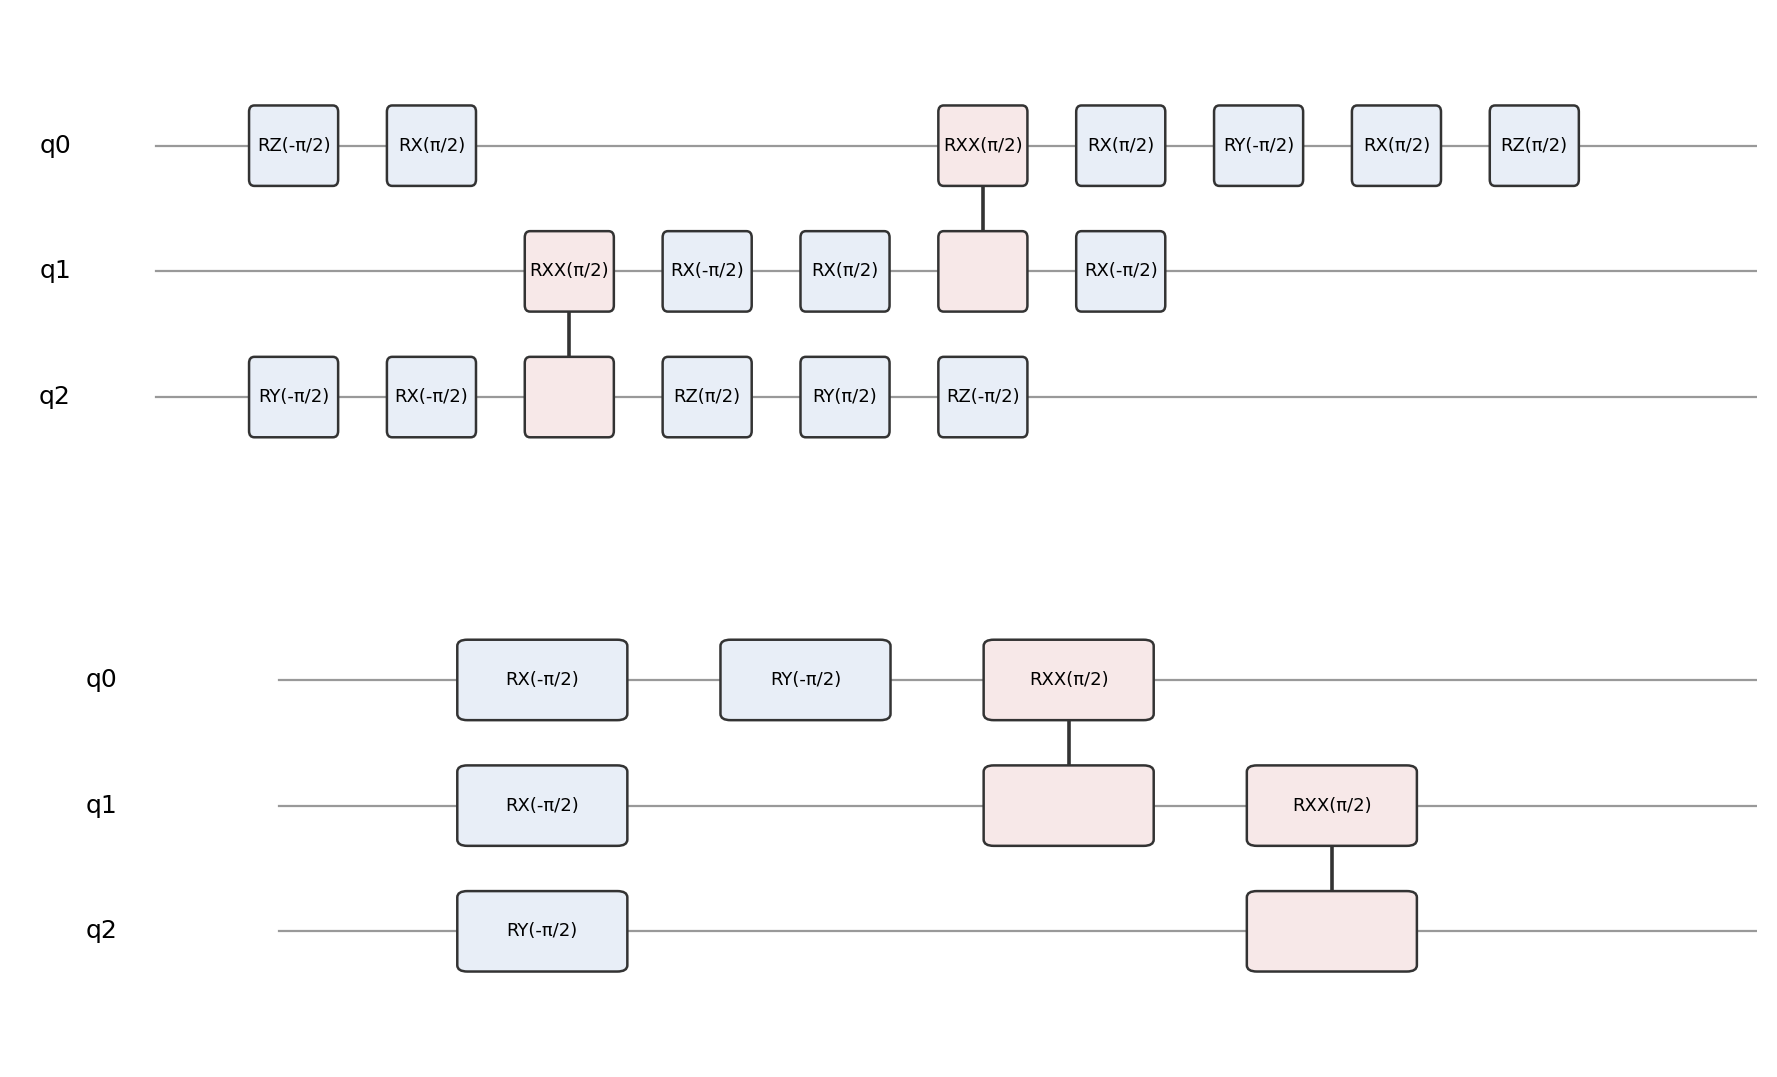
\includegraphics[width=0.62\linewidth]{../figures/paper/our_figure1_4_example_reduction.png}
    \caption{A random 16-gate ion-trap circuit reduced to 6 gates by the
    exact engine, verified unitary-equivalent to machine precision.}
    \label{fig:example}
\end{figure}

\begin{figure}[H]
    \centering
    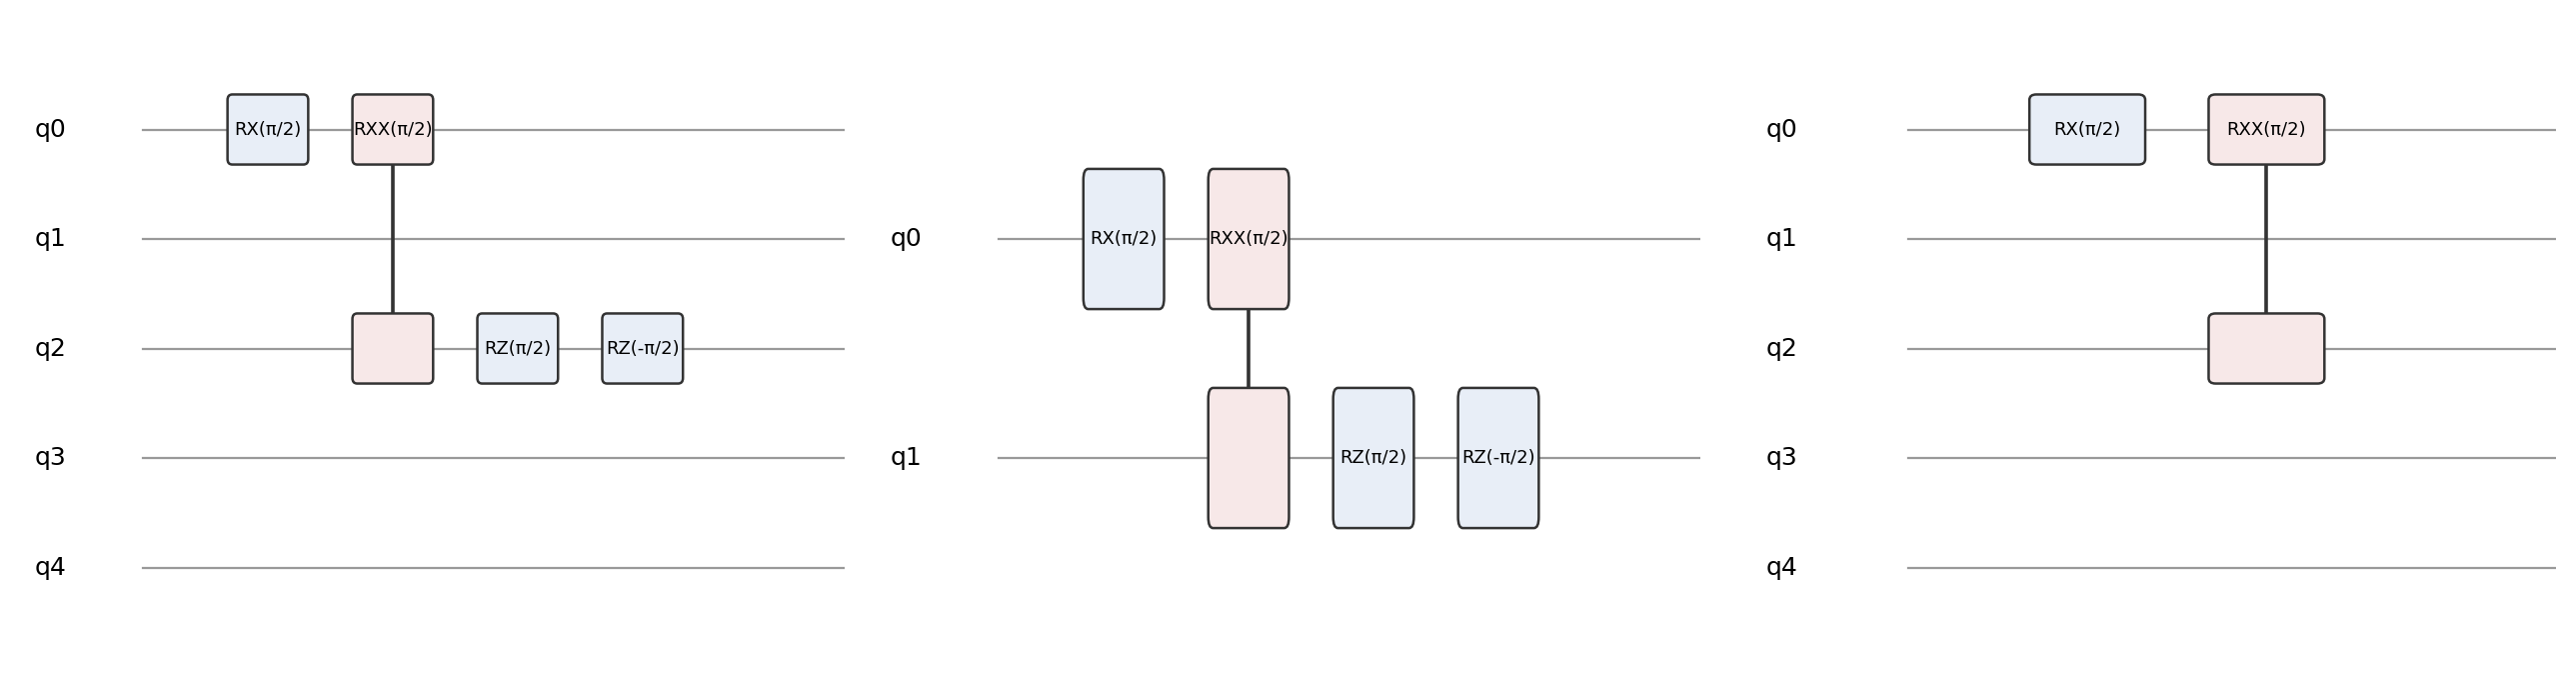
\includegraphics[width=0.68\linewidth]{../figures/paper/our_figure7_wire_reduction.png}
    \caption{A block touching two of a five-wire register's qubits is
    remapped to local coordinates, matched against the two-wire compute
    graph, and the shorter replacement is lifted back onto the original
    wires. Two adjacent $RZ$ rotations of opposite sign cancel, so the
    lifted-back block is two gates shorter than the input.}
    \label{fig:wire}
\end{figure}

Compute graph size is the practical constraint on how deep this search can
go. Figure~\ref{fig:graphgrowth} shows measured node counts for both gate
sets at two and three wires: growth is close to exponential in depth and
faster for larger pools, which is why every configuration in this paper
fixes a depth per wire count rather than searching to a uniform depth.

\begin{figure}[H]
    \centering
    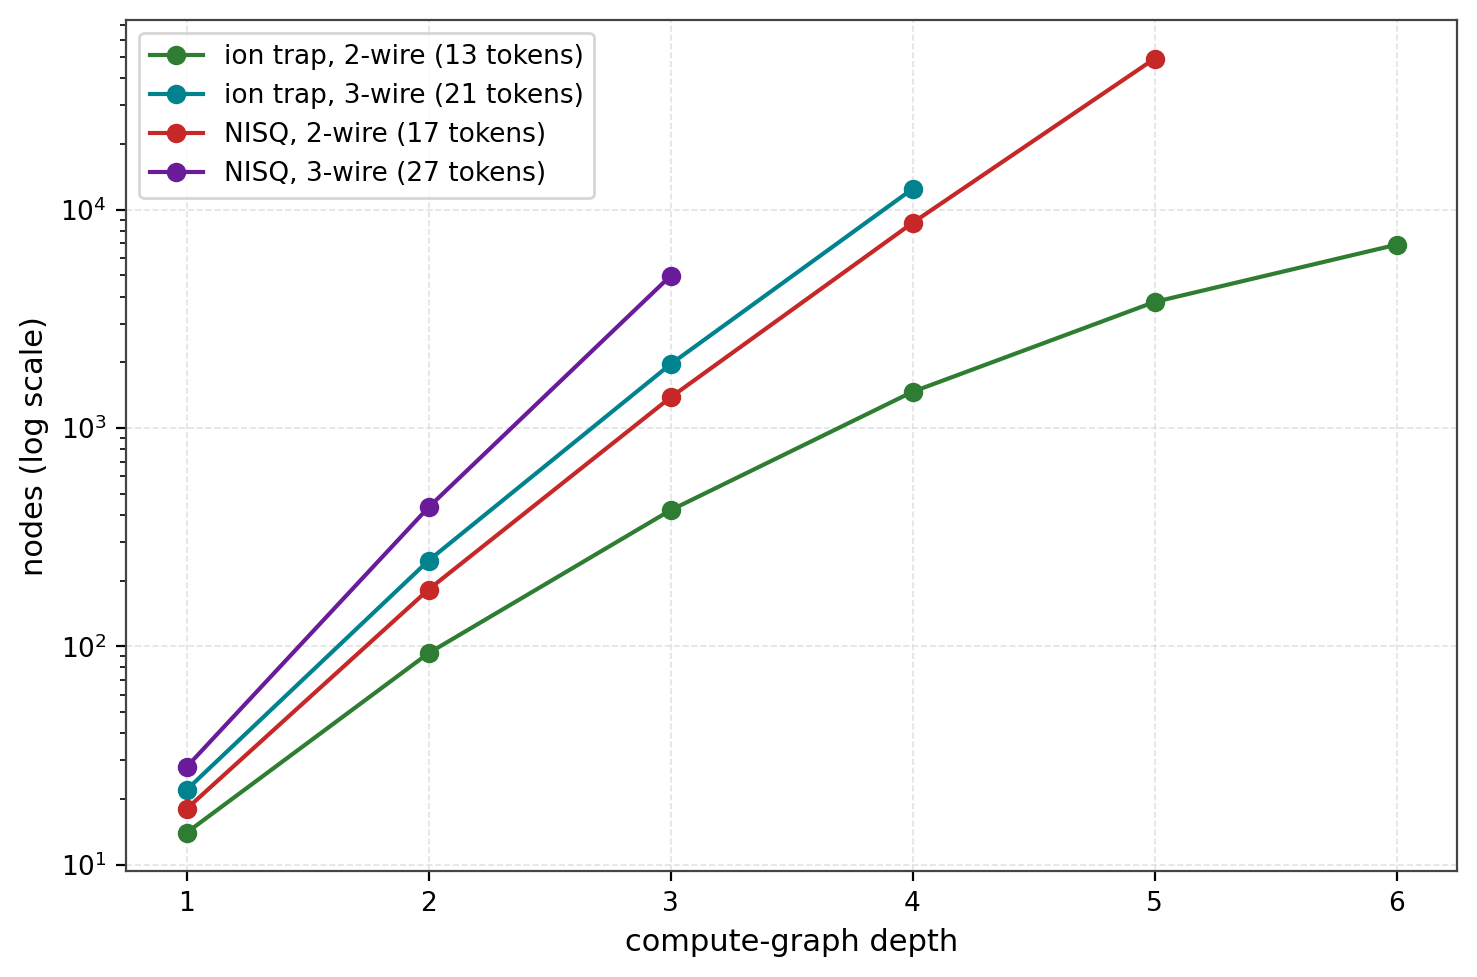
\includegraphics[width=0.58\linewidth]{../figures/paper/our_figure2_compute_graph_growth.png}
    \caption{Measured compute-graph node counts against depth, both gate
    sets, two and three active wires (log scale). The NISQ pool is larger
    at every wire count because it includes both $\pm\pi/2$ and
    $\pm\pi/4$ rotations, so its graphs grow faster and are correspondingly
    more expensive to build to a given depth.}
    \label{fig:graphgrowth}
\end{figure}

\subsection{An exact engine for Clifford pools}
\label{sec:exact}

The ion-trap pool, RX, RY and RZ at $\pm\pi/2$ together with RXX at
$\pi/2$, is entirely Clifford. Every element of the Clifford group is
determined up to global phase by its conjugation action on the Pauli
generators \cite{Gottesman1998Heisenberg}, and that action is representable
exactly as a binary symplectic matrix with an integer phase vector
\cite{AaronsonGottesman2004,BravyiMaslov2021Clifford}. We build the
ion-trap compute graph over this signed-tableau representation rather than
over floating-point unitaries: two circuits collide in the graph if and
only if they induce the same tableau, with no rounding and no tolerance
parameter anywhere in the comparison. A replacement found this way is
equivalent to the block it replaces by construction, not by having passed
a numerical check.

This buys two things beyond correctness. Table lookups become integer
operations instead of floating-point matrix comparisons, so the same
hardware builds noticeably deeper graphs in the same time. And because
equivalence is exact, the search can freely explore equal-length rewrites
that only change which gates are used, which is what makes the cost-aware
objective below possible without accumulating floating-point error over
many replacements.

\subsection{A cost-aware objective}

Local term replacement as originally specified minimizes total gate
count. On real hardware, single-qubit and two-qubit gates do not cost the
same: two-qubit gates dominate both error rate and duration on essentially
every current platform \cite{Preskill2018NISQ,Cross2019QuantumVolume}. We
add an objective that orders candidate replacements lexicographically by
(two-qubit gate count, total length) rather than by length alone. Because
the exact engine can safely accept equal-length rewrites, this objective
can trade a single-qubit gate for another single-qubit gate purely to
remove a two-qubit gate elsewhere in the resulting chain, a class of
improvement invisible to a length-only search.

\subsection{Search and structural passes}

The full reduction pipeline (Figure~\ref{fig:pipeline}) is: an optional
algebraic pre-pass that fuses adjacent same-axis rotations and cancels
back-to-back two-qubit gates using exact angle arithmetic; clustering of
single-qubit gates between two-qubit barriers and collapse of same-wire
runs against the one-wire graph; an exhaustive sweep of the database over
every window up to a fixed length; a deterministic reordering pass,
described below, together with randomized transport shuffling of gates
across ones they commute with; and an escape step that resamples an
irreducible window with a structurally different equivalent word before
re-sweeping, accepted only if it strictly shortens the circuit. The whole
loop repeats to a fixpoint or until the time budget expires, and every
output is verified against the input unitary before being reported. This
is the pipeline diagnosed in Sections~\ref{sec:results}--\ref{sec:more-candidates};
Section~\ref{sec:burst} adds an optional first phase for the NISQ pool
specifically, ported directly from the published method's own reference
implementation, that this pipeline's own final cleanup pass still runs
after.

\begin{figure}[H]
    \centering
    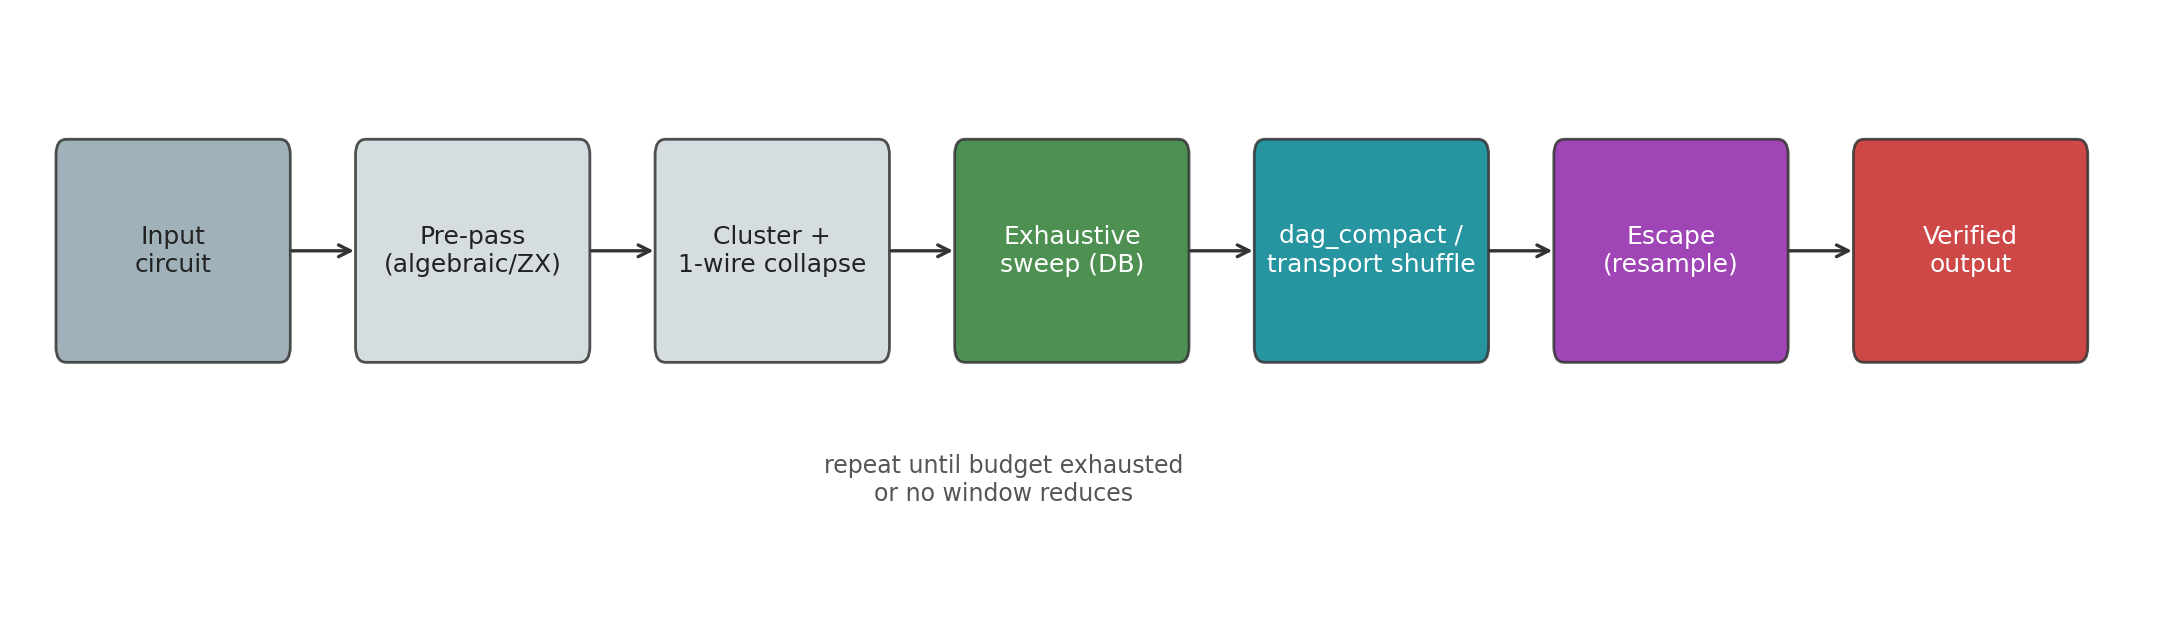
\includegraphics[width=0.70\linewidth]{../figures/paper/our_figure3_pipeline.png}
    \caption{The reduction pipeline. Structural passes run once; the
    sweep, reordering and escape steps repeat until the circuit stops
    shrinking or the time budget is exhausted.}
    \label{fig:pipeline}
\end{figure}

\subsection{Deterministic block reordering}
\label{sec:dag}

The exhaustive sweep only finds a reduction if the gates it needs are
already adjacent in the flat gate list, and otherwise depends on the
randomized shuffle bringing them together by chance. We add a
deterministic alternative in the spirit of two-qubit block collection in
production compilers \cite{JavadiAbhari2024Qiskit}, generalized to
$k$-wire blocks: the circuit's per-wire dependency structure, in which a
gate depends on the most recent gate touching each of its wires, gives a
partial order on the gate list, and any two gates that act on disjoint
wires can be freely swapped without changing the circuit's unitary.
Reordering the gate list so that every maximal block touching at most
three wires becomes contiguous is therefore always a valid reordering, and
it exposes windows to the sweep that the randomized shuffle would
otherwise only find by chance.

An earlier version of this pipeline re-ran the reordering on every
iteration of the stochastic loop, alongside the randomized shuffle, and
made results measurably worse rather than better (ion trap: mean 87.4
against 83.3 gates over 7 seeds at a 10-second budget). The reordering is a
pure function of the gate list, so re-applying it to an already-reordered,
otherwise-unchanged list is a no-op; interleaved with the randomized
shuffle inside the loop, it displaced roughly half of the loop's
diversity-generating passes on the common case where nothing had changed
since the last reordering, without contributing anything in return.
Running it once, as a pre-pass before the stochastic loop begins rather
than inside it, fixes this and is the configuration used everywhere below;
we return to what this reveals about the search itself in
Section~\ref{sec:dag-result}.

\subsection{Incremental window construction}
\label{sec:incremental}

The exhaustive sweep tries every window length from the block-length cap
down to two at each position, and both engines originally rebuilt the
tried length's local representation, the embedded unitary for the numeric
engine, the signed tableau for the exact engine, from scratch for each
length independently: a cap of eight costs $2+3+\cdots+8=35$ gate
applications where eight would do. We instead extend one gate at a time,
from length one up to the cap, reusing the previous length's
partially-built representation and widening it only when a gate introduces
a wire the window has not yet touched (a Kronecker product with identity
for the numeric engine's matrix; two new rows inserted at the position the
tableau's own constructor would place them for the exact engine, so the
resulting key stays comparable to the graph's stored nodes). The
wire-to-local-index assignment this produces differs from the
ascending-real-wire-number one the rest of the pipeline uses, but the
compute graph is built by exploring every pool gate on every local wire
and pair uniformly, so it is symmetric under any relabeling of its own
local wires; an exhaustive per-window comparison against the original
construction confirms the two engines never disagree on the achievable
length (or, for the exact engine's bounded Pareto-alternatives cache, on
the achievable length and two-qubit count). Under the same wall-clock
budget this raises search throughput substantially, on the cost-aware
ion-trap protocol mean passes completed per circuit rise several-fold, and
the results reported in Table~\ref{tab:ion} already reflect it.

\section{Experimental setup}
\label{sec:setup}

We evaluate against the hundred-circuit protocol from
\cite{Rosenhahn2025Optimization}: four qubits, length-300 random circuits,
one hundred circuits per gate set with identical inputs across every
method compared, and a fixed per-circuit time budget. Ion-trap circuits
sample uniformly from the gate pool; NISQ circuits weight CZ twice as
heavily as RX or RZ, matching the input composition the original
protocol reports. Reduced circuits are verified against their input,
exactly for the all-Clifford ion-trap pool and to $10^{-5}$ up to global
phase otherwise; every run reported below passes verification.

Two independent transpiler baselines are run on the same inputs: qiskit
\cite{JavadiAbhari2024Qiskit} at optimization levels 1 through 3, and
BQSKit \cite{Younis2021BQSKit}, where available, at levels 2 through 4.
Where BQSKit is not installed in the evaluation environment its row is
omitted rather than estimated.

\section{Results}
\label{sec:results}

\subsection{Ion trap: exceeding the published baseline}
\label{sec:ion-result}

Table~\ref{tab:ion} reports mean gate counts, by type, over the
hundred-circuit protocol. Both of our reducers beat the published result
on total gate count and, more importantly for hardware, on two-qubit gate
count.

\begin{table}[H]
\centering
\caption{Ion-trap pool, mean gates over 100 identical circuits (std.\ in
parentheses). ``Baseline'' is the published result for the same protocol
\cite{Rosenhahn2025Optimization}.}
\label{tab:ion}
\begin{tabular}{lrrrrr}
\toprule
method & RX & RY & RZ & RXX & total \\
\midrule
input             & 78 (7)      & 83 (8)      & 78 (7)      & 59 (7)      & 298 \\
baseline \cite{Rosenhahn2025Optimization} & 10 (3) & 29 (6) & 29 (5) & 43 (8) & 111 \\
qiskit L1--L3     & \multicolumn{4}{c}{---}                              & 160.8--167.1 \\
\textbf{ours, length-minimizing} & 2.4 (1.3)  & 18.2 (5.2) & 17.2 (4.7) & 28.2 (6.7) & \textbf{66.1 (14.5)} \\
\textbf{ours, cost-aware}        & 2.9 (1.6)  & 18.8 (5.1) & 19.2 (5.0) & \textbf{25.9 (5.1)} & \textbf{66.7 (12.9)} \\
\bottomrule
\end{tabular}
\end{table}

The improvement is large and consistent, not an artifact of a few
favorable circuits: a one-sample $t$-test of the hundred per-circuit
results against the published mean of 111 gives $t=-34.3$
($p=1.0\times10^{-56}$, Cohen's $d=-3.4$, 95\% CI $[64.1,69.3]$) for the
cost-aware objective. Figure~\ref{fig:ion} places this alongside the
qiskit baselines. The cost-aware objective removes roughly two further
RXX gates than the length-only objective at a comparable total, exactly
the behavior it is designed to produce: an equal-length rewrite that
trades a two-qubit gate for a single-qubit one is invisible to a search
that only counts length.

\begin{figure}[H]
    \centering
    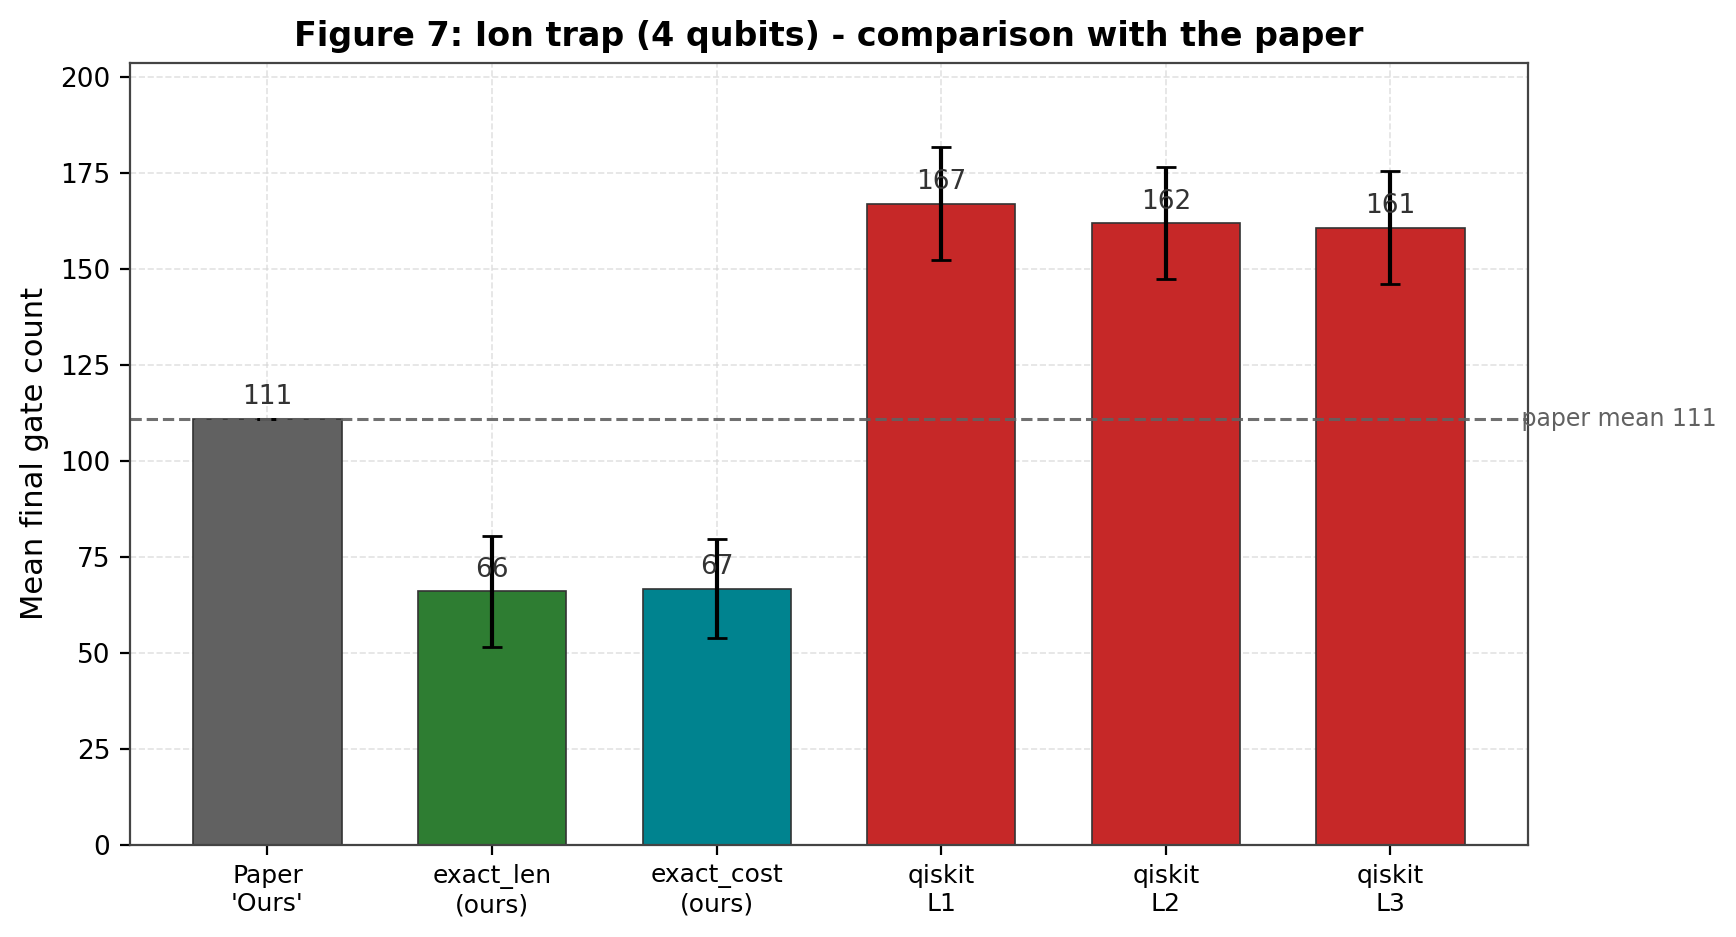
\includegraphics[width=0.60\linewidth]{../figures/paper/figure7_comparison_ion_trap.png}
    \caption{Ion-trap total gate count, mean over 100 circuits. Error bars
    are one standard deviation.}
    \label{fig:ion}
\end{figure}

Figure~\ref{fig:composition} breaks the reduction down by gate type for
both pools. On ion trap, RX drops furthest in relative terms (96\%),
because the search can freely rewrite any single-qubit sequence into a
canonical short form once a block's overall Clifford action is fixed.
Figure~\ref{fig:twoqubit} isolates the two-qubit count specifically, the
metric most directly tied to circuit fidelity on real hardware: 25.9 RXX
gates against the baseline's 43, a 40\% reduction that did not require
sacrificing total length.

\begin{figure}[H]
    \centering
    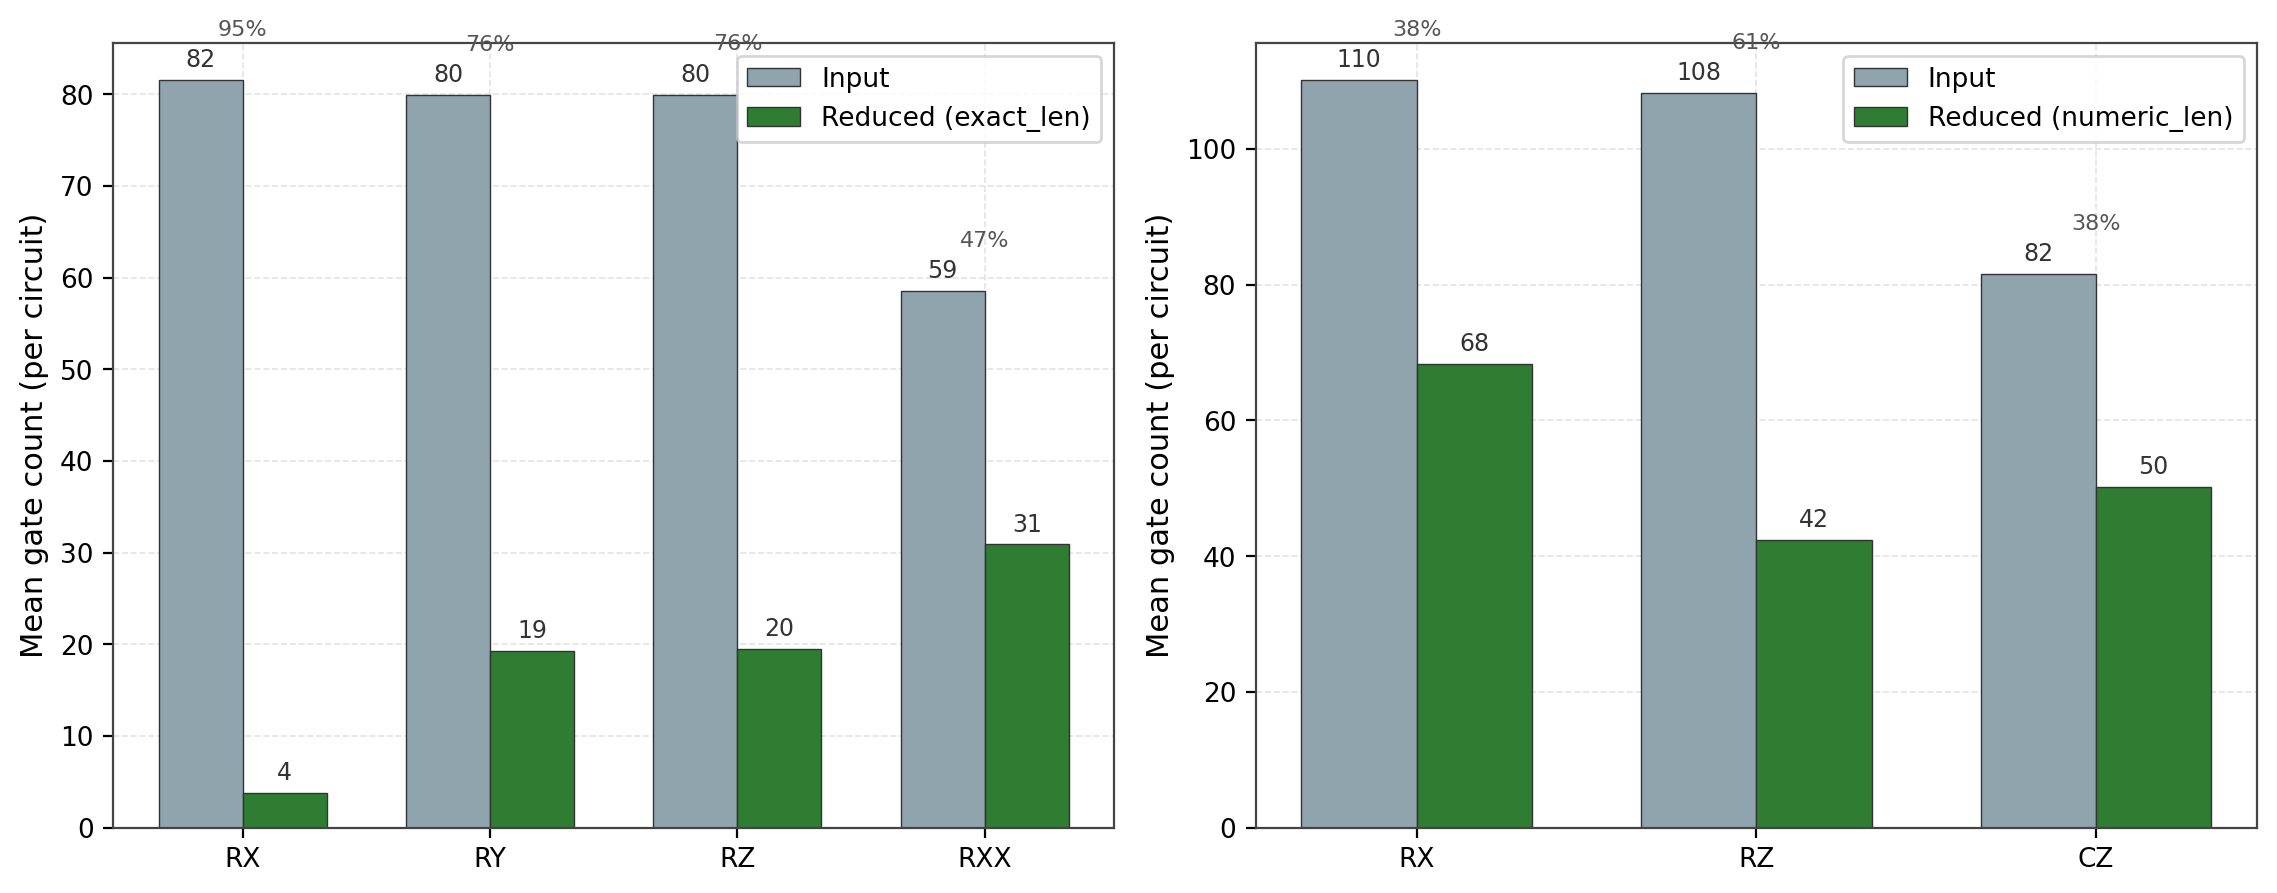
\includegraphics[width=0.72\linewidth]{../figures/paper/figure3_pipeline.png}
    \caption{Gate composition of input versus reduced circuits, mean over
    the comparison runs, both gate sets. Percentages give the relative
    reduction per gate type.}
    \label{fig:composition}
\end{figure}

\begin{figure}[H]
    \centering
    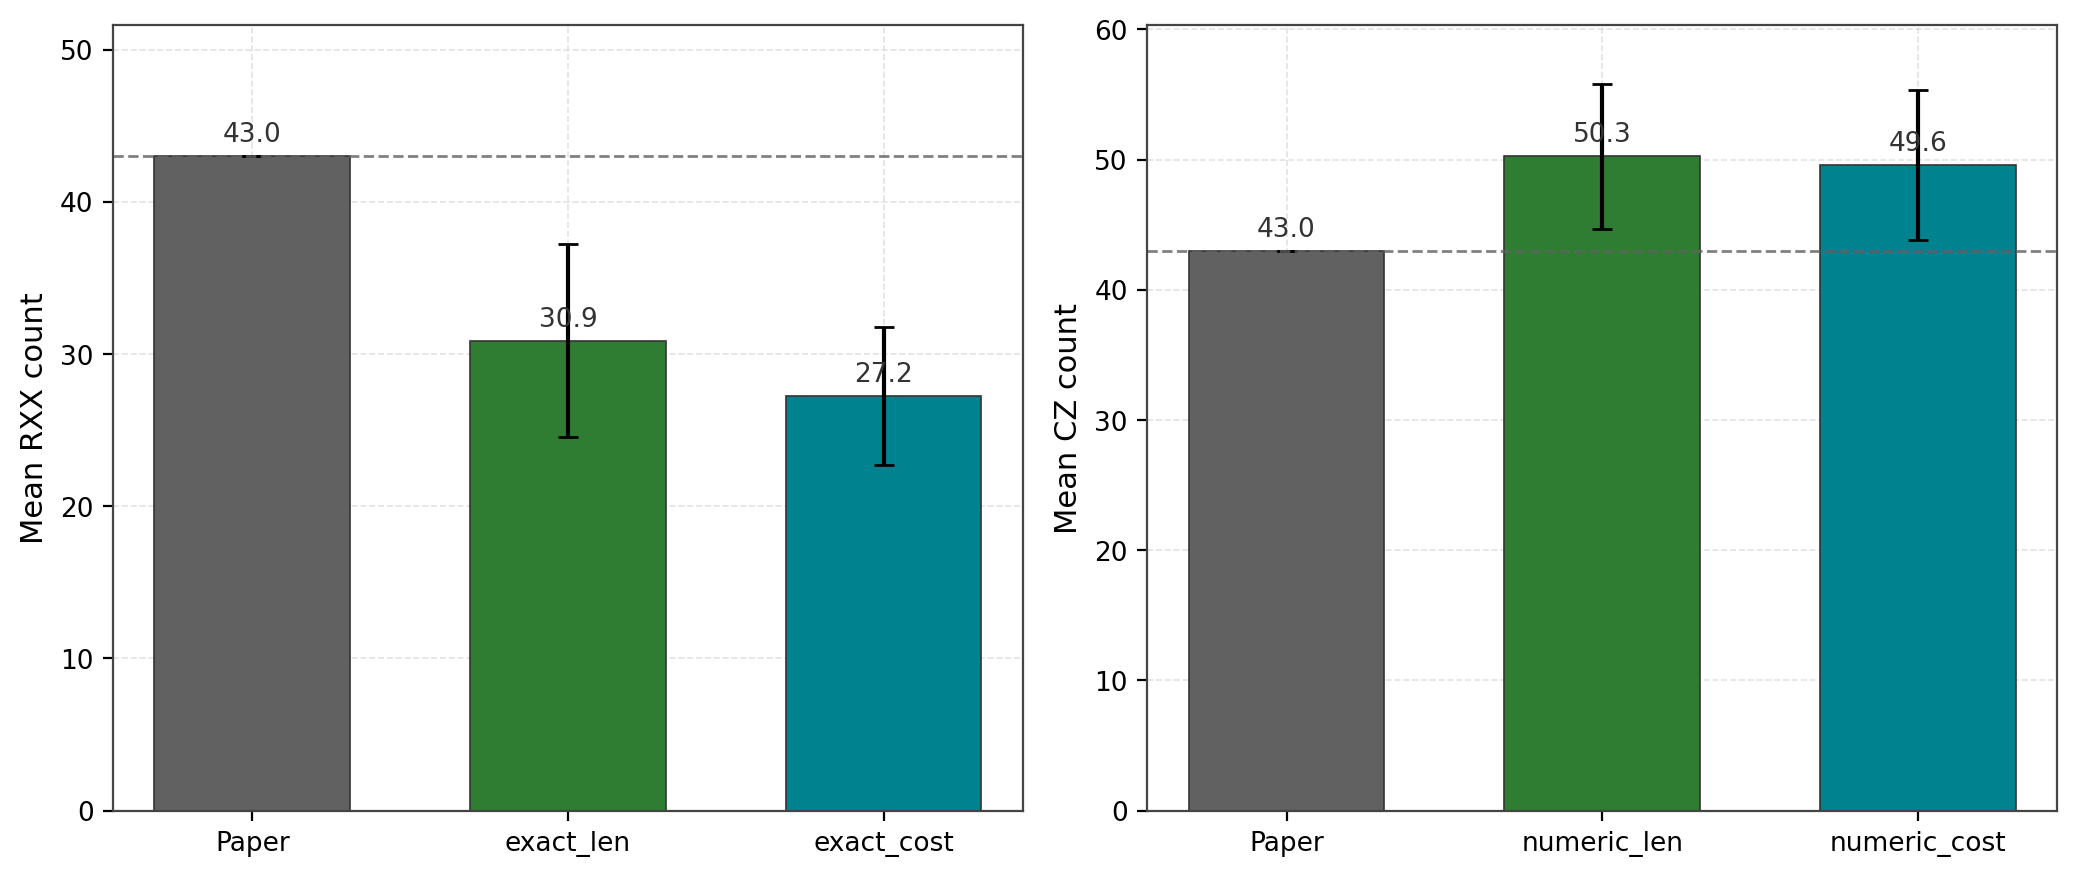
\includegraphics[width=0.72\linewidth]{../figures/paper/figure9_two_qubit_counts.png}
    \caption{Two-qubit gate counts, the hardware-relevant metric, for both
    gate sets against the published baseline (dashed line).}
    \label{fig:twoqubit}
\end{figure}

One caveat applies to this comparison. Our qiskit baselines (167.1, 162.0,
160.8 for levels 1 through 3) come in below the published qiskit baselines
(196, 204, 204) on the same input composition, most plausibly because of a
qiskit version difference between the two studies. The improvement margin
above should be read with this in mind; the NISQ baseline fidelity check
in the next section is considerably tighter and supports the comparison
framework more directly.

\subsection{NISQ: a gap remains}
\label{sec:nisq-result}

The same protocol on the NISQ pool tells a different story
(Table~\ref{tab:nisq}, Figure~\ref{fig:nisq}). Our reducer, run with an
RZ-across-CZ transport pass to a fixpoint and a hybrid mode that routes any
fully-Clifford window to the exact engine, ends at a mean of 160.5 gates
against the published 107 with the exhaustive sweep described in
Section~\ref{sec:method}; Sections~\ref{sec:discussion}--\ref{sec:burst}
report a systematic attempt to explain that gap, one finding from which
(the matlab\_demo-faithful burst reducer, Section~\ref{sec:burst}) is
adopted as the new default and lowers this to 155.1, still against the
same published 107 -- the diagnosis below is carried out, and should be
read, against the pre-burst 160.5 figure it was actually run against.

\begin{table}[H]
\centering
\caption{NISQ pool, mean gates over 100 identical circuits (std.\ in
parentheses). The last two rows are the current default, added in
Section~\ref{sec:burst}; every other section of this paper discusses the
exhaustive-sweep rows above them, which is what was actually being
diagnosed.}
\label{tab:nisq}
\begin{tabular}{lrrrr}
\toprule
method & RX & RZ & CZ & total \\
\midrule
input             & 109 (9)    & 109 (8)    & 82 (8)     & 300 \\
baseline \cite{Rosenhahn2025Optimization} & 45 (6) & 19 (4) & 43 (6) & 107 \\
qiskit L1--L3     & \multicolumn{3}{c}{---}               & 157.8--201.8 \\
ours, exhaustive sweep, length-minimizing & 68.3 (5.9) & 42.3 (5.1) & 50.3 (5.6) & 160.9 (12.8) \\
ours, exhaustive sweep, cost-aware        & 68.6 (6.1) & 42.3 (5.2) & 49.6 (5.8) & 160.5 (13.4) \\
\textbf{ours, burst (default), length-minimizing} & 67.5 (6.0) & 38.7 (4.8) & 49.1 (5.5) & \textbf{155.3 (12.5)} \\
\textbf{ours, burst (default), cost-aware}        & 67.6 (6.1) & 38.6 (4.9) & 48.9 (5.5) & \textbf{155.1 (12.4)} \\
\bottomrule
\end{tabular}
\end{table}

\begin{figure}[H]
    \centering
    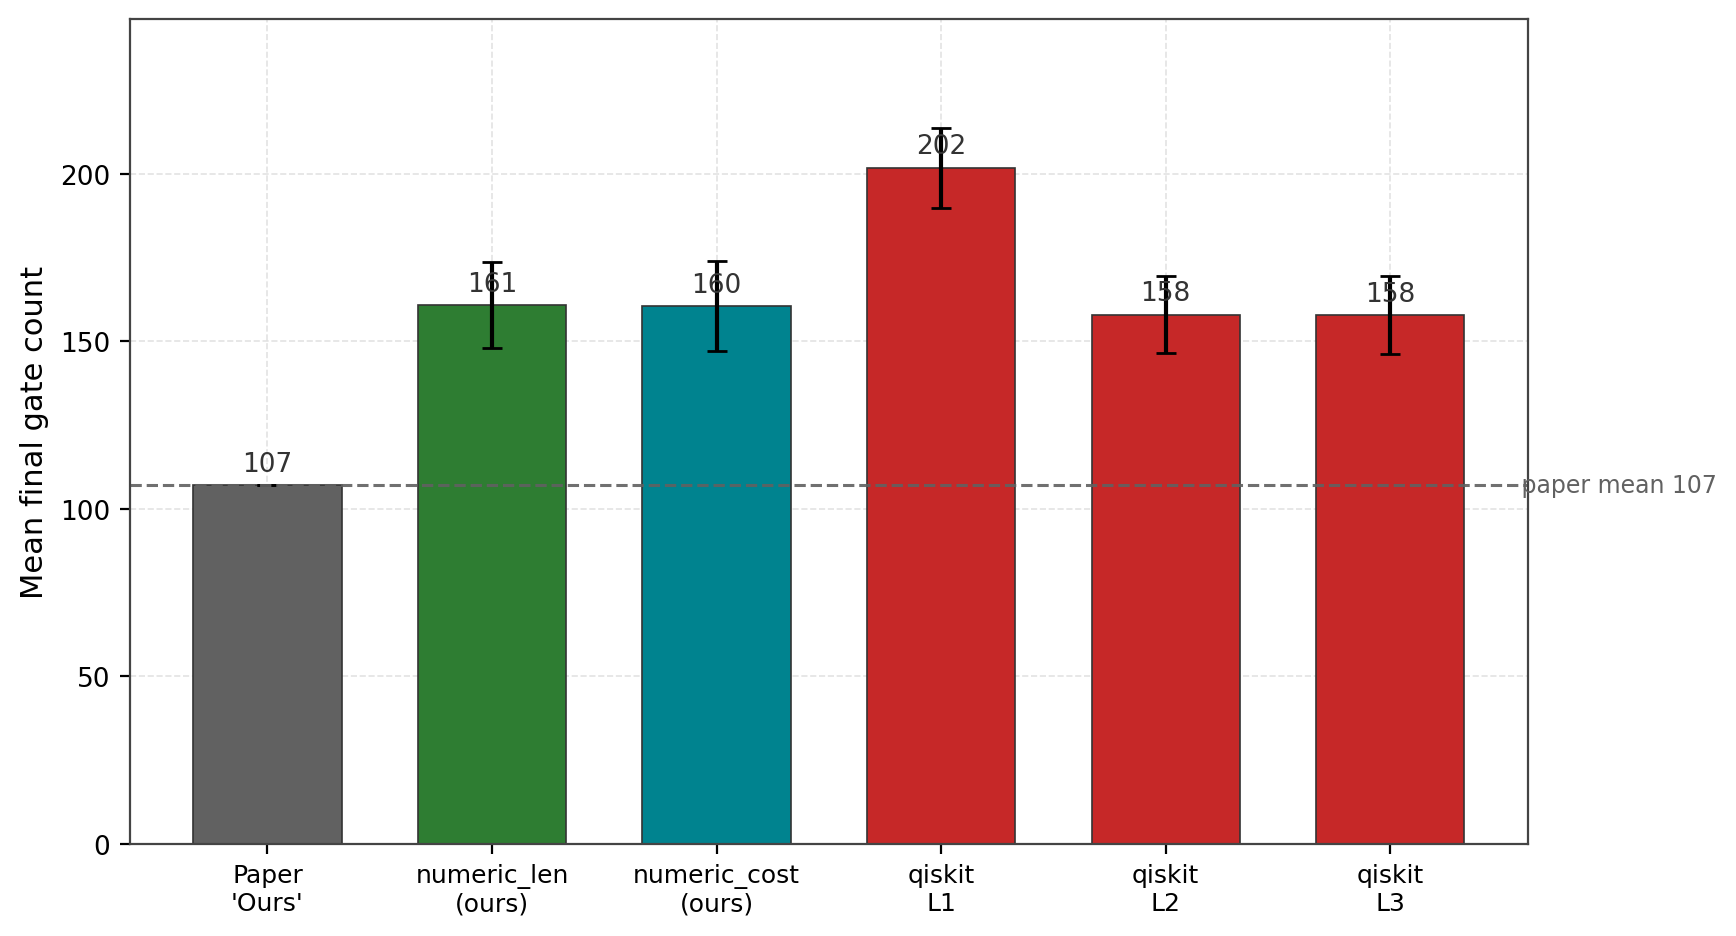
\includegraphics[width=0.60\linewidth]{../figures/paper/figure8_comparison_nisq.png}
    \caption{NISQ total gate count, mean over 100 circuits, against qiskit
    and the published baseline.}
    \label{fig:nisq}
\end{figure}

Two checks establish that this comparison is fair rather than an artifact
of a mismatched setup. The input composition matches the published Table 7
row closely (our RX/RZ/CZ means of 109/109/82 against the published
108/109/82), and our qiskit baselines (157.8 at both levels 2 and 3,
201.8 at level 1) match the published qiskit baselines (149 and 196) far
more closely than on the ion-trap protocol. The gap is also statistically
unambiguous: $t=+39.7$ ($p=1.3\times10^{-62}$, $d=4.0$) for the exhaustive-sweep
cost-aware objective against the published mean of 107 (the pre-burst
figure the diagnosis below was actually run against). The remainder of
this paper treats this gap as the central open question and reports a
systematic attempt to explain it.

A second, narrower question is why the cost-aware objective, which clearly
helps on ion trap (Section~\ref{sec:ion-result}), barely moves NISQ's
two-qubit count at all (Table~\ref{tab:nisq}: 49.6 against 50.3 CZ gates,
within run-to-run noise across independent runs). Probing every reducible
window across five 200-gate NISQ circuits found the mechanism itself
intact: cost-aware and length-only lookups agree exactly whenever a
genuine reduction exists (844/844 matched candidates, zero discrepancies),
and raising the stored-alternatives cap from 4 to 32 (never hit at that
width; the deepest alternative list actually reached was 27) surfaced zero
additional same-length, lower-two-qubit-count candidates across 1267
reducible windows. The cost-aware objective works as designed at the
lookup level; it has nothing to select between. The cause is structural:
the all-Clifford ion-trap pool packs only two angles per rotation, so many
distinct token sequences collide onto the same compute-graph node, and
that collision is exactly what populates a node's alternative-factorization
list; the larger four-angle NISQ pool needed to reach the non-Clifford
$\pi/4$ rotations is correspondingly sparser at the same depth, and its
nodes rarely have more than one factorization to choose from at all, let
alone a two-qubit-cheaper one.

\section{Diagnosing the NISQ gap}
\label{sec:discussion}

A gap this large, roughly 50\% at the total-length level, has an
explanation, and finding it is the point of running a method against a
strong published baseline rather than reporting the discrepancy and moving
on. We worked through six candidate causes in turn.

\textbf{Input composition.} Already addressed above: the generated input
circuits match the published composition to within noise.

\textbf{Compute-graph depth.} Our default NISQ configuration already
builds a three-wire graph to depth 5, matching the deepest configuration
reported in the source method's own growth data. Rebuilding the
three-wire graph one level deeper, to depth 6, and the two-wire graph to
depth 8, using a disk-backed store since the resulting graphs exceed a
laptop's RAM, narrows the gap by only about 2\% (Table~\ref{tab:deep}).
Depth alone was not the bottleneck.

\begin{table}[H]
\centering
\caption{NISQ total gate count against increasingly deep compute graphs,
100 circuits each.}
\label{tab:deep}
\begin{tabular}{lcc}
\toprule
database & length-minimizing & cost-aware \\
\midrule
default (3-wire depth 5, 4-wire depth 4) & 160.9 (12.8) & 160.5 (13.4) \\
deeper (3-wire depth 6, 4-wire depth 4)  & 157.3 (12.8) & 157.2 (12.6) \\
\bottomrule
\end{tabular}
\end{table}

\textbf{Search-time budget.} The exhaustive sweep reaches the same end
length at a 10-second budget as at 60 seconds, and running several
independent restarts and keeping the best barely moves the mean. The
search converges to a fixed point well within budget; it does not run out
of time.

\textbf{Search-loop structure.} \label{sec:sampling}
Local term replacement as originally specified is not one algorithm but
three, and its strongest variant gates a random-sampling loop with a
learned classifier that skips lookups predicted to fail. We reimplemented
both the plain random-sampling loop and its classifier-gated variant and
ran them at equal budget against our exhaustive sweep on the same NISQ
inputs (Table~\ref{tab:loop}). Neither improves on the sweep; gating makes
the loop measurably worse, because the classifier suppresses genuinely
reducible lookups (replacements fall from 78.2 to 69.0 per run) while its
own decision overhead cuts the number of loop iterations by an order of
magnitude. The loop structure is not what the published numbers depend
on, at least not on this implementation of the underlying compute graph.

\begin{table}[H]
\centering
\caption{Search-loop variants, reimplemented, six NISQ circuits, 10-second
budget each.}
\label{tab:loop}
\begin{tabular}{lrrr}
\toprule
method & end length (mean) & replacements & database lookups \\
\midrule
exhaustive sweep     & 161.5 & --- & --- \\
random sampling      & 168.2 & 78.2 & 44{,}166 \\
classifier-gated sampling & 179.5 & 69.0 & 2{,}293 attempted, 994 skipped \\
\bottomrule
\end{tabular}
\end{table}

\textbf{Window discovery.} \label{sec:dag-result}
The deterministic block-reordering pass of Section~\ref{sec:dag} gives an
independent way to test whether the search is simply failing to find the
windows the database could reduce. On ion trap, at a fixed short budget,
it shortens circuits by 4.5 to 10\% relative to the unreordered baseline;
at the protocol's own 30-second budget that narrows to 3.6\% as the
stochastic loop has time to catch up on its own. On NISQ, under the
identical treatment, the effect is 0.2 to 1.7\% at short budgets and
effectively zero, $-0.1\%$, at 30 seconds, despite the reordering pass
exposing substantially larger candidate windows on NISQ than on ion trap
(mean block length 6 to 14 gates, against the sweep's default 8-gate cap).
More windows reach the database; almost none of them reduce. This is
evidence against the search missing windows and for the database itself
lacking coverage.

\textbf{Compute-graph node-key precision.} The published method merges
duplicate compute-graph nodes using a $10^{-5}$ numerical tolerance on the
unitary comparison; our implementation instead keys nodes by an exact hash
of the unitary rounded to ten decimal places, tighter by five orders of
magnitude. If floating-point drift on deep chains were pushing two
genuinely equal unitaries to round differently at that precision, our
graph would be spuriously larger than it should be, undercounting coverage
in a way that would compound with depth, consistent with the small effect
depth has above. Rebuilding the same NISQ graph at five different
precision levels down to four decimal places produces an identical node
count at every one, at every depth tested. Double-precision error on these
short, well-conditioned products is orders of magnitude below even a
coarse rounding threshold; this is not the mechanism.

\subsection{Testing the depth hypothesis further: a deeper four-wire graph}
\label{sec:deep5}

With five candidates ruled out, we are left with database factorization
coverage: for a nontrivial fraction of NISQ blocks that the published
method evidently reduces, ours does not find a shorter equivalent chain at
any depth built so far. One structural asymmetry stood out from the
ablations above. Every NISQ configuration used in Table~\ref{tab:deep}
caps the four-wire compute graph at depth 4, even though the evaluation
circuits are exactly four qubits wide: a block spanning the full register
can only ever be reduced by the four-wire graph, regardless of how deep
the three-wire graph goes. We built a four-wire graph one level deeper, to
depth 5 (1,912,349 nodes, up from 167,449 at depth 4), specifically to
test this.

Benchmarking this graph exposed a second, purely engineering, issue.
Our comparison harness distributes circuits across worker processes, and
the disk-backed compute-graph store, necessary because the combined
four-graph database exceeds 11 million nodes, must reopen its own SQLite
connections in each worker rather than share a parent process's connection
across a fork. The initial implementation reloaded the store from disk on
every individual circuit rather than once per worker process; a single
reload measures 154 seconds, so across two hundred per-circuit tasks,
reload time alone came to dominate wall-clock time by roughly two orders
of magnitude over the intended per-circuit search budget, leaving the
deeper graph with less actual search time than the shallower one and
worse resulting numbers despite its greater coverage. Caching the loaded
store once per worker process, keyed identically to the existing
per-process cache used for the in-memory backend, restores per-task
timing to the intended budget; the failure mode is general to any
local-search circuit optimizer benchmarked against a compute graph too
large to fit in memory under process parallelism, not specific to this
codebase.

Table~\ref{tab:deep5} reports the depth-5 four-wire result under the
corrected harness, on the full hundred-circuit protocol at the paper's own
60-second budget.

\begin{table}[H]
\centering
\caption{NISQ total gate count, default database versus the depth-5
four-wire graph, both under the corrected per-process caching, 100
circuits, 60-second budget.}
\label{tab:deep5}
\begin{tabular}{lcc}
\toprule
database & length-minimizing & cost-aware \\
\midrule
default (4-wire depth 4)      & 160.9 (12.8) & 160.5 (13.4) \\
depth-5 four-wire graph       & 160.7 (13.0) & 161.0 (13.1) \\
\bottomrule
\end{tabular}
\end{table}

The deeper graph produces no improvement: both differences are smaller
than one standard error of the mean at this sample size, and the
cost-aware objective is marginally worse rather than better. Four-wire
depth is not the bottleneck either, on top of three-wire depth already
shown to account for only about 2\% of the gap (Table~\ref{tab:deep}).
This rules out depth along both wire-count axes without resolving the
gap: whatever the published database supports on wide, mixed-rotation
blocks that ours does not, it is not simply a matter of building either
graph deeper, and identifying the specific factorization responsible
remains open.

\subsection{Two more candidates: node-key fragility and reach extension}
\label{sec:more-candidates}

Two further candidates were tested after the six above, neither of which
was suggested by the original diagnostic pass; both are real, and neither
closes the gap.

\textbf{Node-key fragility.} Every place this codebase turns a raw complex
matrix into a hashable compute-graph key picks a single largest-magnitude
entry as the global-phase reference. This is fragile: two different token
chains that reach the same unitary up to global phase are computed via
independent floating-point multiplication paths, and for a pool rich in
diagonal gates (RZ, CZ -- exactly NISQ) many entries legitimately tie or
nearly tie in magnitude, so different paths can round to different entries
as ``the largest,'' each carrying a different phase, silently fragmenting
one physical compute-graph node into several. Replacing the single-entry
pivot with a whole-matrix phase reference (the sum of every entry, far
less sensitive to any one coordinate's tie-breaking) merges 21--32\% more
nodes on the NISQ pool (2-wire depth 5: 123{,}689 $\to$ 84{,}220 nodes;
3-wire depth 4: 83{,}820 $\to$ 66{,}261), verified safe by checking every
newly-merged group for genuine unitary equivalence across 213{,}000+
sampled node pairs (zero false collisions). Despite this real, substantial
reduction in node fragmentation, a controlled comparison at matched
seeds and budget shows no measurable change in circuit-level results
(159.9 $\to$ 162.1 length-minimizing, 170.7 $\to$ 170.8 cost-aware,
both within noise): the recovered coverage turns out to be almost
entirely redundant with what the fragmented scheme already found in
practice. The fix is kept in the codebase regardless, since it is a
genuine, verified, zero-downside correctness improvement (smaller graphs,
faster builds at fixed memory), but it is a seventh ruled-out cause, not
an eighth data point for the depth hypothesis.

\textbf{Reach extension.} A bidirectional (meet-in-the-middle) database
lookup already existed in this codebase's own tooling: undo one trailing
gate from a block's target unitary by left-multiplying with a pool gate's
inverse, and check whether the residual is within the compute graph's
direct reach, extending effective coverage by one gate at the cost of one
extra lookup per pool token. At a short, smoke-test budget this looks like
a clear regression (NISQ mean $+12.0$ gates); the reason is that each
extended lookup costs $|\mathcal{P}|$ ($17$--$27$ for this pool) times as
many queries as a direct one, so the reducer completes zero full sweep
passes before the budget expires. At a realistic 45-second budget it does
find genuine additional matches -- 12{,}033 extended hits a direct lookup
missed, out of 54{,}418 total, on six circuits -- but the per-lookup
overhead still dominates: 3--4 completed passes against the plain sweep's
30+, and the net effect remains slightly worse (163.5 $\to$ 168.5 gates,
$+3.1\%$). Extra reach exists and is real; it is not worth its own cost
at this pool's branching factor, an eighth ruled-out cause.

\subsection{A ninth attempt: porting the reference implementation's own loop}
\label{sec:burst}

The MATLAB reference implementation released alongside
\cite{Rosenhahn2025Optimization} (\texttt{matlab\_demo/QCOptimDemo} in
this repository) is not merely a gate-set specification: its
\texttt{optimCodeGMode1DComp.m} implements a complete reduction loop, and
it differs from this codebase's exhaustive sweep in several concrete,
previously-untested ways. Windows are rejection-sampled to at most three
wires -- its own compute graph is 3-wire only, so it never attempts a
full four-qubit-register window at all, unlike the four-wire graph this
codebase built specifically to cover that case
(Section~\ref{sec:deep5}). Window length is a single random draw in
$[1,\min(\text{remaining},7)]$, not an exhaustive try-every-length,
longest-first sweep. Structural collapse is far weaker: its
\texttt{simplereduce.m} only cancels an adjacent pair whose combined
unitary is exactly the identity, nothing like this codebase's full
single-wire collapse against the complete one-wire graph or its algebraic
pre-pass. No MATLAB or Octave installation was available to run the
reference code directly (nor would Octave supply the MATLAB Quantum
Computing Support Package functions the demo depends on), so this loop
was ported to Python faithfully, gate for gate, against this codebase's
own NISQ database, and named \texttt{reduce\_matlab\_burst}.

Every individual mechanism above is weaker than this codebase's own
exhaustive sweep, but each attempt is far cheaper, so within a fixed
wall-clock budget it completes one to two orders of magnitude more raw
attempts (measured: 100{,}000+ attempts at a 30--60 second budget, against
15--90 completed sweep passes for the same budget). Screening the split
between the two loops (running the ported loop for a fraction of the
budget before handing off to the exhaustive pipeline for whatever
remains, at fractions $0, 0.15, 0.3, 0.5, 0.75, 1$) found the two extremes
dominate every mixture in between; spending the entire budget on the
ported loop wins outright, with the existing pipeline's own unconditional
final structural-plus-sweep cleanup pass still applied afterward. This
configuration, exposed as \texttt{reduce\_circuit}'s \texttt{burst\_frac}
parameter and defaulted to $1.0$ for the NISQ pool, is adopted as this
codebase's new default and is what Table~\ref{tab:nisq}'s last two rows
report.

\begin{table}[H]
\centering
\caption{NISQ total gate count, exhaustive sweep (the previous default)
versus the matlab\_demo-faithful burst reducer (the new default),
identical 100 seeds, identical hybrid setting, full official protocol.}
\label{tab:burst}
\begin{tabular}{lccc}
\toprule
method & exhaustive sweep & burst (new default) & paired $\Delta$ \\
\midrule
length-minimizing & 160.9 (12.8) & 155.3 (12.5) & $-5.6$ ($-3.4\%$) \\
cost-aware         & 160.5 (13.4) & 155.1 (12.4) & $-5.4$ ($-3.3\%$) \\
\bottomrule
\end{tabular}
\end{table}

\begin{figure}[H]
    \centering
    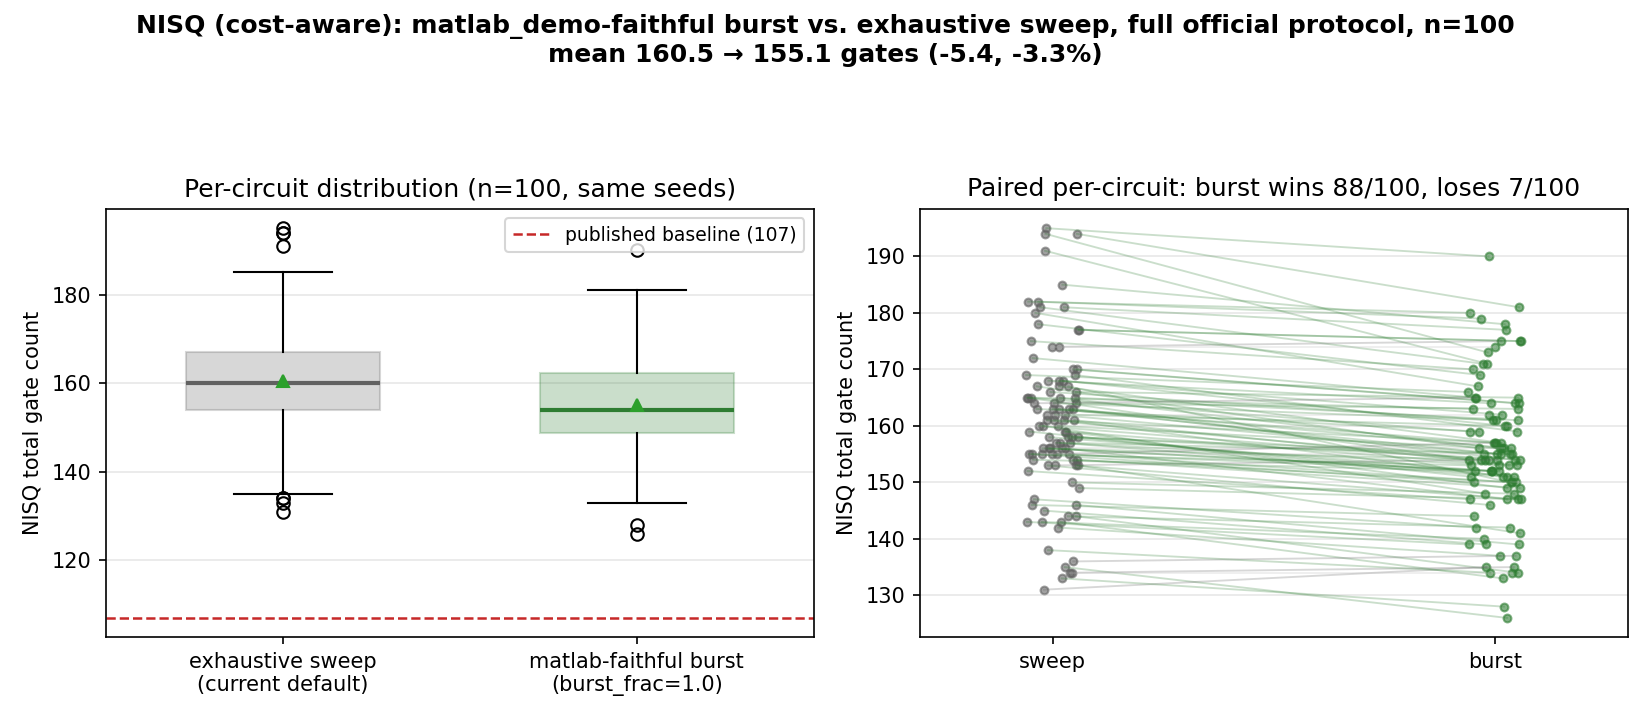
\includegraphics[width=0.95\linewidth]{../figures/figure_matlab_burst_nisq_cost.png}
    \caption{NISQ cost-aware total gate count, exhaustive sweep versus the
    matlab\_demo-faithful burst reducer, $n=100$, identical seeds. Left:
    per-circuit distribution against the published baseline. Right: paired
    per-circuit change, colored by direction.}
    \label{fig:burst}
\end{figure}

The improvement is real and consistent, not a few favorable circuits: a
paired $t$-test against the exhaustive-sweep result on the same seeds
gives $t=-13.7$ ($p=1.5\times10^{-24}$, Cohen's $d=-1.37$) for
length-minimizing and $t=-12.3$ ($p=9.2\times10^{-22}$, $d=-1.23$) for
cost-aware; the burst reducer wins outright on 91/100 and 88/100 seeds
respectively, and every one of the 200 resulting circuits (100 seeds
$\times$ 2 objectives) passes unitary verification. Two things should be
said about what this result is not. It does not close the gap to the
published baseline: 155.1 remains a $45\%$ shortfall against 107, not a
$50\%$ one. And it was found empirically, not derived from a specific
diagnosed mechanism -- the most plausible account is that raw iteration
throughput of cheap, individually weaker stochastic moves outweighs fewer,
more careful ones under this search's particular time budget, a
possibility the six-hypothesis diagnostic study above did not consider
because ``how many attempts fit in the budget'' is a different axis from
any of input composition, database depth, time budget, loop \emph{choice}
among the paper's own three variants, window discovery, or node-key
precision. It is reported here as a real, load-bearing, but modest
addition on top of an otherwise still-open question, not as a resolution
of it.

\subsection{Why the ion-trap pool behaves differently}

The two pools are not just harder or easier versions of the same problem.
The NISQ pool's $\pm\pi/4$ rotations are not Clifford, so the exact
engine in Section~\ref{sec:exact} does not apply to it at all, and its
compute graph is intrinsically larger at every depth
(Figure~\ref{fig:graphgrowth}) for the same reason it is harder to
search. The published method's NISQ advantage, whatever its exact
mechanism, is doing something our database construction does not yet
replicate on that harder pool.

\subsection{A mixed Clifford/non-Clifford ion-trap pool: a boundary case}
\label{sec:mixed-ion}

Both protocols evaluated above fix a fully-Clifford ion-trap pool and a
NISQ pool that is Clifford only through a small sub-pool routed to the
exact engine by the hybrid database (Section~\ref{sec:method}). To test
whether the method's ion-trap advantage survives a richer, more
transpiler-realistic gate set, we built a third pool: RX, RY, RZ at
$\pm\pi/2$, $\pm\pi/4$, and $\pm\pi/8$ (mixing Clifford and non-Clifford
rotations in the same pool), with RXX fixed at the native $\pi/2$
entangler as before. The same hybrid routing applies: windows entirely
within the $\pm\pi/2$ sub-pool go to the exact engine, everything else to
the numeric one.

This pool's branching factor grows sharply with wire count relative to
either evaluated protocol: 18/37/57/78 tokens at one through four wires,
against plain ion-trap's 6/13/21/30. Direct calibration of the compute
graph's own growth (not the paper's evaluation protocol) found the
one-wire graph alone reaches 545{,}000 nodes by depth 6 and 25.6 million by
depth 8, a 47$\times$ jump for two additional levels. The depths usable
within a comparable time budget are consequently much shallower than
either protocol above: 6/4/4/3 by wire count, against ion-trap's 12/10/7/5.

On this pool, at these depths, the method loses to plain qiskit, not just
to BQSKit: an exploratory run (3 circuits, 4-qubit, length-300, 5-second
budget) reduced to a mean of 166.0 gates (length-minimizing) and 167.7
gates (cost-aware), against qiskit's 115.7--119.0 across optimization
levels 1--3. Every reduced circuit still verifies exactly against its
input (bit-exact where the exact engine applies, numeric-verified
elsewhere), so the shortfall is a search-quality gap, not a correctness
one. Given the sample size this is a directional finding, not a
statistically powered one, but the gap (166 against 117, roughly 42\%) is
far larger than anything attributable to three circuits' worth of sampling
noise.

This is the boundary condition the ion-trap result above does not reveal
on its own: the local term-replacement approach's edge comes from deep
compute graphs, and pool size trades directly against reachable depth
under a fixed build budget. Ion trap's small, all-Clifford pool affords
depth 12 at one wire; this richer pool's larger branching factor limits
the same budget to depth 6. A generic transpiler that does not depend on a
precomputed lookup table pays no such price for a richer gate set, and
outperforms this method here as a direct consequence. Closing this gap
would need either a way to reach deep effective coverage without paying
for it in raw branching factor -- plausibly the same database
factorization question left open for NISQ (Section~\ref{sec:discussion})
-- or a fundamentally different technique for large pools, not a deeper
build of the current one.

\section{Limitations}

BQSKit baselines are omitted from the main hundred-circuit tables
(Tables~\ref{tab:ion}, \ref{tab:nisq}) for tractability, not availability;
a separate, smaller ($n=30$) head-to-head against BQSKit levels 2--4 is
reported in the repository's README rather than in this paper, since it
was not run on identical machinery throughout the project and BQSKit
level 4 in particular failed unitary verification for every ion-trap
circuit tested, an unresolved issue on our side rather than a claim about
BQSKit itself. The
hardware validation reported for the published method, comparing reduced
and unreduced circuits on real IBM devices, is outside the scope of this
study; every result in this paper is a unitary-verified simulation. The published
method's single-circuit six-qubit and fifteen-qubit examples are not part
of the hundred-run protocol evaluated here. All experiments ran on a
single consumer machine (8 cores, 16\,GB RAM); the disk-backed compute
graphs used for the deeper NISQ configurations exist specifically to make
that constraint tractable, at the cost of slower builds and the
per-process caching discipline described in Section~\ref{sec:deep5}.

\section{Conclusion}

The additions in Section~\ref{sec:method}, an exact engine, a cost-aware
objective, deterministic block reordering, and incremental window
construction, are enough on their own to exceed a strong published
baseline on an all-Clifford gate set, on both total length and the
two-qubit count that governs hardware fidelity. On a
NISQ gate set outside the exact engine's reach, the same infrastructure
falls short of that baseline; systematically eliminating eight candidate
explanations in turn, including compute-graph depth tested independently
on the three-wire and four-wire graphs, a node-keying fragility fix, and
a bidirectional reach extension, localizes the cause to a database
factorization limit that persists regardless of how deep either graph is
built, and identifying the specific factorization responsible is left
open. A ninth attempt, faithfully porting the published method's own
MATLAB reference implementation rather than a further ablation of this
codebase's own machinery, does help: adopted as the new default, it
narrows the gap by $3$--$3.5\%$ ($p<10^{-21}$, $n=100$,
Section~\ref{sec:burst}) without closing it, and is reported as exactly
that -- a real, modest, empirically-found improvement layered on an
otherwise still-open question, not a resolution of it. The per-process
caching defect the deeper-graph experiment surfaced is worth taking away
independently of this method: it applies to any local-search circuit
optimizer benchmarked against a compute graph too large to fit in memory.

\section*{Data availability}
Source code, benchmark data, and figures supporting the findings of this
study are available from the corresponding author upon reasonable
request.

\bibliographystyle{plain}
\begin{thebibliography}{99}

\bibitem{Rosenhahn2025Optimization}
B.~Rosenhahn, T.~J.~Osborne, and C.~Hirche.
\newblock Optimization driven quantum circuit reduction.
\newblock \emph{New Journal of Physics}, 27:104509, 2025.

\bibitem{RosenhahnTobias2023MCGS}
B.~Rosenhahn and T.~J.~Osborne.
\newblock Monte Carlo graph search for quantum circuit optimization.
\newblock \emph{Physical Review A}, 108:062615, 2023.

\bibitem{RosenhahnHirche2024NormalizingFlows}
B.~Rosenhahn and C.~Hirche.
\newblock Quantum normalizing flows for anomaly detection.
\newblock \emph{Physical Review A}, 110:022443, 2024.

\bibitem{Gottesman1998Heisenberg}
D.~Gottesman.
\newblock The Heisenberg representation of quantum computers.
\newblock arXiv:quant-ph/9807006, 1998.

\bibitem{AaronsonGottesman2004}
S.~Aaronson and D.~Gottesman.
\newblock Improved simulation of stabilizer circuits.
\newblock \emph{Physical Review A}, 70:052328, 2004.

\bibitem{BravyiMaslov2021Clifford}
S.~Bravyi and D.~Maslov.
\newblock Hadamard-free circuits expose the structure of the Clifford
group.
\newblock \emph{IEEE Transactions on Information Theory}, 67(7):4546--4563,
2021.

\bibitem{NielsenChuang2010}
M.~A.~Nielsen and I.~L.~Chuang.
\newblock \emph{Quantum Computation and Quantum Information}.
\newblock Cambridge University Press, 2010.

\bibitem{Preskill2018NISQ}
J.~Preskill.
\newblock Quantum computing in the NISQ era and beyond.
\newblock \emph{Quantum}, 2:79, 2018.

\bibitem{Arute2019Supremacy}
F.~Arute et al.
\newblock Quantum supremacy using a programmable superconducting processor.
\newblock \emph{Nature}, 574:505--510, 2019.

\bibitem{Cross2019QuantumVolume}
A.~W.~Cross, L.~S.~Bishop, S.~Sheldon, P.~D.~Nation, and J.~M.~Gambetta.
\newblock Validating quantum computers using randomized model circuits.
\newblock \emph{Physical Review A}, 100:032328, 2019.

\bibitem{Amy2014TDepth}
M.~Amy, D.~Maslov, and M.~Mosca.
\newblock Polynomial-time T-depth optimization of Clifford+T circuits via
matroid partitioning.
\newblock \emph{IEEE Transactions on Computer-Aided Design of Integrated
Circuits and Systems}, 33(10):1476--1489, 2014.

\bibitem{Nam2018Automated}
Y.~Nam, N.~J.~Ross, Y.~Su, A.~M.~Childs, and D.~Maslov.
\newblock Automated optimization of large quantum circuits with continuous
parameters.
\newblock \emph{npj Quantum Information}, 4:23, 2018.

\bibitem{Maslov2017IonTrap}
D.~Maslov.
\newblock Basic circuit compilation techniques for an ion-trap quantum
machine.
\newblock \emph{New Journal of Physics}, 19:023035, 2017.

\bibitem{ZulehnerPalerWille2018}
A.~Zulehner, A.~Paler, and R.~Wille.
\newblock An efficient methodology for mapping quantum circuits to the IBM
QX architectures.
\newblock \emph{IEEE Transactions on Computer-Aided Design of Integrated
Circuits and Systems}, 38(7):1226--1236, 2018.

\bibitem{BlumRoli2003Metaheuristics}
C.~Blum and A.~Roli.
\newblock Metaheuristics in combinatorial optimization: overview and
conceptual comparison.
\newblock \emph{ACM Computing Surveys}, 35(3):268--308, 2003.

\bibitem{JavadiAbhari2024Qiskit}
A.~Javadi-Abhari et al.
\newblock Quantum computing with Qiskit.
\newblock arXiv:2405.08810, 2024.

\bibitem{Sivarajah2020Tket}
S.~Sivarajah, S.~Dilkes, A.~Cowtan, W.~Simmons, A.~Edgington, and R.~Duncan.
\newblock t$|$ket$\rangle$: a retargetable compiler for NISQ devices.
\newblock \emph{Quantum Science and Technology}, 6(1):014003, 2020.

\bibitem{Younis2021BQSKit}
E.~Younis, C.~C.~Iancu, W.~Lavrijsen, M.~Davis, and E.~Smith.
\newblock Berkeley Quantum Synthesis Toolkit (BQSKit) v1.
\newblock Lawrence Berkeley National Laboratory, 2021.
\newblock Available at \url{https://bqskit.lbl.gov}.

\bibitem{Martyniuk2024QASSurvey}
D.~Martyniuk, J.~Jung, and A.~Paschke.
\newblock Quantum architecture search: a survey.
\newblock arXiv:2406.06210, 2024.

\bibitem{Zhu2023QASSurvey}
W.~Zhu, J.~Pi, and Q.~Peng.
\newblock A brief survey of quantum architecture search.
\newblock In \emph{Proceedings of the 6th International Conference on
Algorithms, Computing and Systems (ICACS '22)}. ACM, 2023.

\bibitem{Zhang2021NeuralPredictorQAS}
S.-X.~Zhang, C.-Y.~Hsieh, S.~Zhang, and H.~Yao.
\newblock Neural predictor based quantum architecture search.
\newblock \emph{Machine Learning: Science and Technology}, 2:045027, 2021.

\bibitem{Zhang2022DifferentiableQAS}
S.-X.~Zhang, C.-Y.~Hsieh, S.~Zhang, and H.~Yao.
\newblock Differentiable quantum architecture search.
\newblock \emph{Quantum Science and Technology}, 7:045023, 2022.

\bibitem{He2024TrainingFreeQAS}
Z.~He, X.~Deng, S.~Zheng, L.~Li, and W.~Situ.
\newblock Training-free quantum architecture search.
\newblock In \emph{Proceedings of the AAAI Conference on Artificial
Intelligence}, volume 38, pages 12430--12438, 2024.

\bibitem{Brandhofer2021Rydberg}
S.~Brandhofer, I.~Polian, and H.~P.~Büchler.
\newblock Optimal mapping for near-term quantum architectures based on
Rydberg atoms.
\newblock In \emph{Proceedings of the IEEE/ACM International Conference on
Computer-Aided Design (ICCAD)}, pages 1--7, 2021.

\bibitem{Datta2022_2DMapping}
K.~Datta, I.~Kole, A.~Sengupta, and R.~Drechsler.
\newblock Mapping quantum circuits to 2-dimensional quantum architectures.
\newblock \emph{INFORMATIK}, 2022.

\bibitem{Datta2022_HexMapping}
K.~Datta, I.~Kole, A.~Sengupta, and R.~Drechsler.
\newblock Nearest neighbor mapping of quantum circuits to two-dimensional
hexagonal architecture.
\newblock In \emph{Proceedings of the IEEE 52nd International Symposium on
Multiple-Valued Logic (ISMVL)}, pages 35--42, 2022.

\bibitem{Murali2020TrappedIon}
P.~Murali, D.~C.~Debroy, K.~R.~Brown, and M.~Martonosi.
\newblock Architecting noisy intermediate-scale trapped ion quantum
computers.
\newblock In \emph{Proceedings of the ACM/IEEE 47th Annual International
Symposium on Computer Architecture (ISCA)}, pages 529--542, 2020.

\bibitem{Breiman2001RandomForests}
L.~Breiman.
\newblock Random forests.
\newblock \emph{Machine Learning}, 45:5--32, 2001.

\bibitem{Ashhab2024RandomSearch}
S.~Ashhab, F.~Yoshihara, M.~Tsuji, M.~Sato, and K.~Semba.
\newblock Quantum circuit synthesis via a random combinatorial search.
\newblock \emph{Physical Review A}, 109:052605, 2024.

\bibitem{Davis2020TopologyAware}
M.~G.~Davis, E.~Smith, A.~Tudor, K.~Sen, I.~Siddiqi, and C.~Iancu.
\newblock Towards optimal topology aware quantum circuit synthesis.
\newblock In \emph{Proceedings of the IEEE International Conference on
Quantum Computing and Engineering (QCE)}, pages 223--234, 2020.

\bibitem{Rasconi2019GeneticCompilation}
R.~Rasconi and A.~Oddi.
\newblock An innovative genetic algorithm for the quantum circuit
compilation problem.
\newblock In \emph{Proceedings of the AAAI Conference on Artificial
Intelligence}, volume 33, pages 7707--7714, 2019.

\bibitem{Wauters2020RLOptimization}
M.~M.~Wauters, E.~Panizon, G.~B.~Mbeng, and G.~E.~Santoro.
\newblock Reinforcement-learning-assisted quantum optimization.
\newblock \emph{Physical Review Research}, 2:033446, 2020.

\bibitem{Wu2021HierarchicalSynthesis}
X.-C.~Wu, M.~G.~Davis, F.~T.~Chong, and C.~Iancu.
\newblock Reoptimization of quantum circuits via hierarchical synthesis.
\newblock In \emph{Proceedings of the 2021 International Conference on
Rebooting Computing (ICRC)}, pages 35--46, 2021.

\bibitem{VandeWetering2020ZX}
J.~van~de~Wetering.
\newblock ZX-calculus for the working quantum computer scientist.
\newblock arXiv:2012.13966, 2020.

\bibitem{Riu2024RLZX}
J.~Riu, J.~Nogué, G.~Vilaplana, A.~Garcia-Saez, and M.~P.~Estarellas.
\newblock Reinforcement learning based quantum circuit optimization via
ZX-calculus.
\newblock arXiv:2312.11597, 2024.

\end{thebibliography}

\end{document}
